\documentclass[tikz,border=10pt]{standalone}

\begin{document}

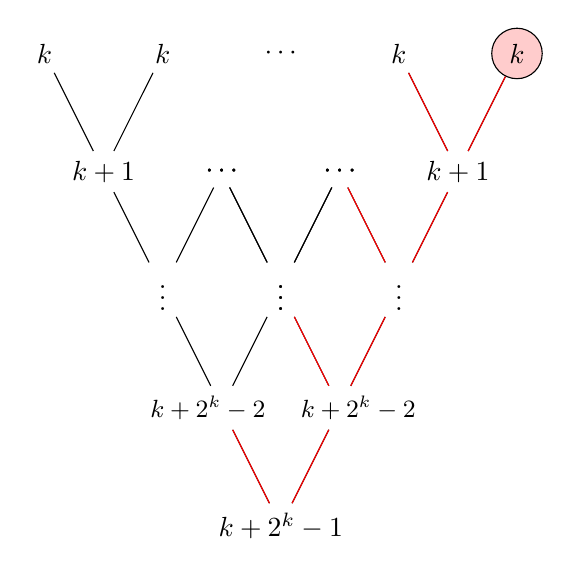
\begin{tikzpicture}[rotate=180]
\node (z){$k+2^k-1$}
  child {node (a) {{\ \ \ \ \small$k+2^k-2$}}
    child {node (b) {$\vdots$}
      child {node (c1) {$k+1$}
        child {node[circle,fill=red!20,draw] (d) {$k$}}
        child {node (e) {$k$}}
      } 
      child {node (a1) {$\cdots$}}
    }
    child {node (g) {$\vdots$}
      child {node {$\cdots$}}
      child {node {$\cdots$}}
    }
  }
  child {node (j) {{\small$k+2^k-2$}\ \ \ \ }
    child {node (k) {$\vdots$}
      child {node {$\cdots$}}
      child {node {$\cdots$}}
    }
  child {node (l) {$\vdots$}
    child {node {$\cdots$}}
    child {node (c){$k+1$}
      child {node (o) {$k$}}
      child {node (p) {$k$}
      }
    }
  }
};
\path (o) -- (e) node (x) [midway] {$\cdots$}
(z) edge[red] (j)
(z) edge[red] (a)
(a) edge[red] (b)
(a) edge[red] (g)
(b) edge[red] (c1)
(b) edge[red] (a1)
(c1) edge[red] (d)
(c1) edge[red] (e)
;
\end{tikzpicture}

\end{document}